\documentclass{article}

\usepackage[utf8]{inputenc}
\usepackage[brazil]{babel}
\usepackage{amsmath, amssymb}
\usepackage{graphicx}
\usepackage{hyperref}
\usepackage{float}
\usepackage{geometry}
\usepackage{caption}
\usepackage{listings}
\usepackage{color}
\usepackage{courier}

\geometry{margin=1in}
\graphicspath{{imagens/}}

\title{Filtro de Kalman}
\author{Eduardo Henrique Basilio de Carvalho}
\date{\today}

\begin{document}

\maketitle

\section*{Questão 1}

\subsection*{a}

\ref{fig:condicoes_iniciais_gaussianas} mostra a nuvem de condições iniciais para o problema.

\begin{figure}[H]
    \centering
    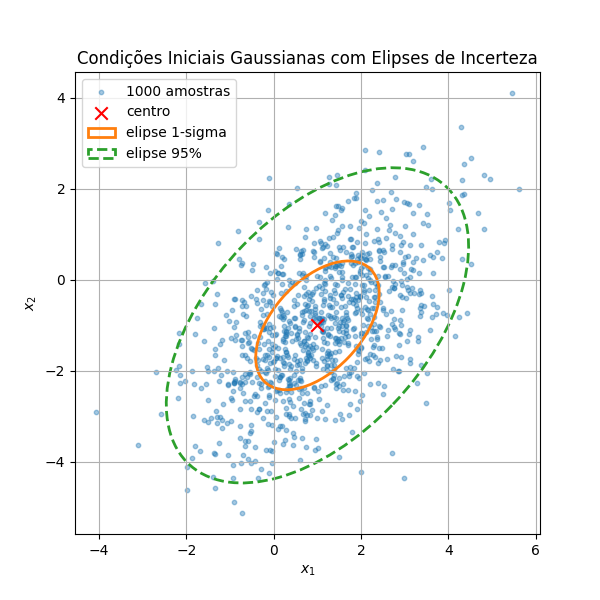
\includegraphics[width=\textwidth]{condicoes_iniciais_gaussianas.png}
    \caption{Nuvem de condições iniciais}
    \label{fig:condicoes_iniciais_gaussianas}
\end{figure}

\subsection*{b}

\ref{fig:nuvem_amostras_propagadas} mostra a nuvem de amostras propagadas pelo modelo dinâmico.

\begin{figure}[H]
    \centering
    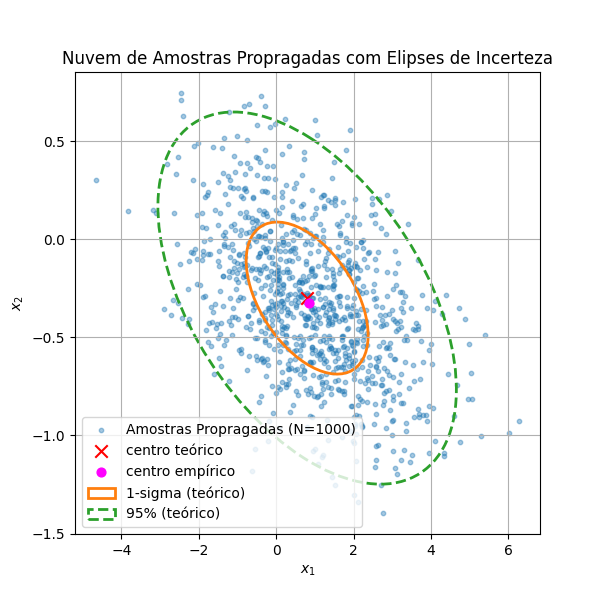
\includegraphics[width=\textwidth]{nuvem_amostras_propagadas.png}
    \caption{Nuvem de amostras propagadas}
    \label{fig:nuvem_amostras_propagadas}
\end{figure}

\subsection*{c}

\ref{fig:correcao_kalman_priori_posteriori} mostra a correção de Kalman para a medição $y_1 = 0.8$.

\begin{figure}[H]
    \centering
    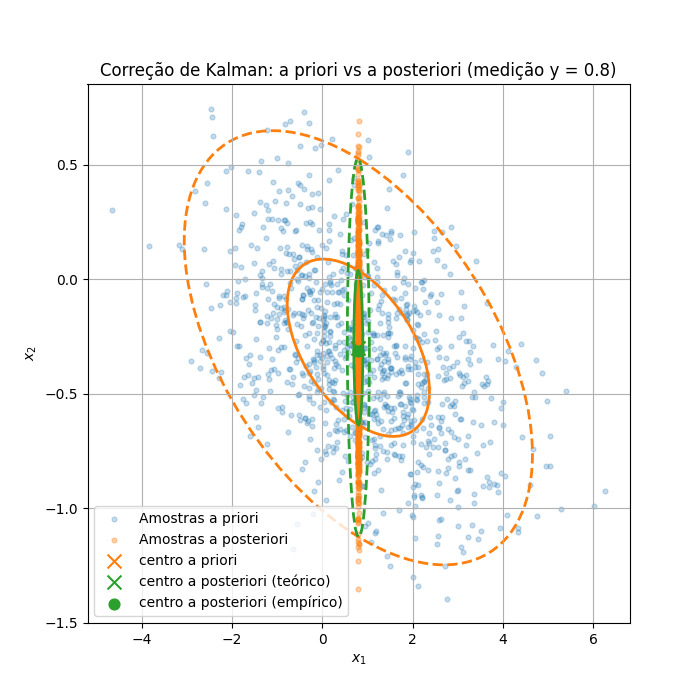
\includegraphics[width=\textwidth]{correcao_kalman_priori_posteriori.png}
    \caption{Correção de Kalman}
    \label{fig:correcao_kalman_priori_posteriori}
\end{figure}

\subsection*{d}

\ref{fig:kf_resultados_1000_passos} mostra a evolução do filtro de Kalman ao longo de 1000 passos e a estima do estado final.

\begin{figure}[H]
    \centering
    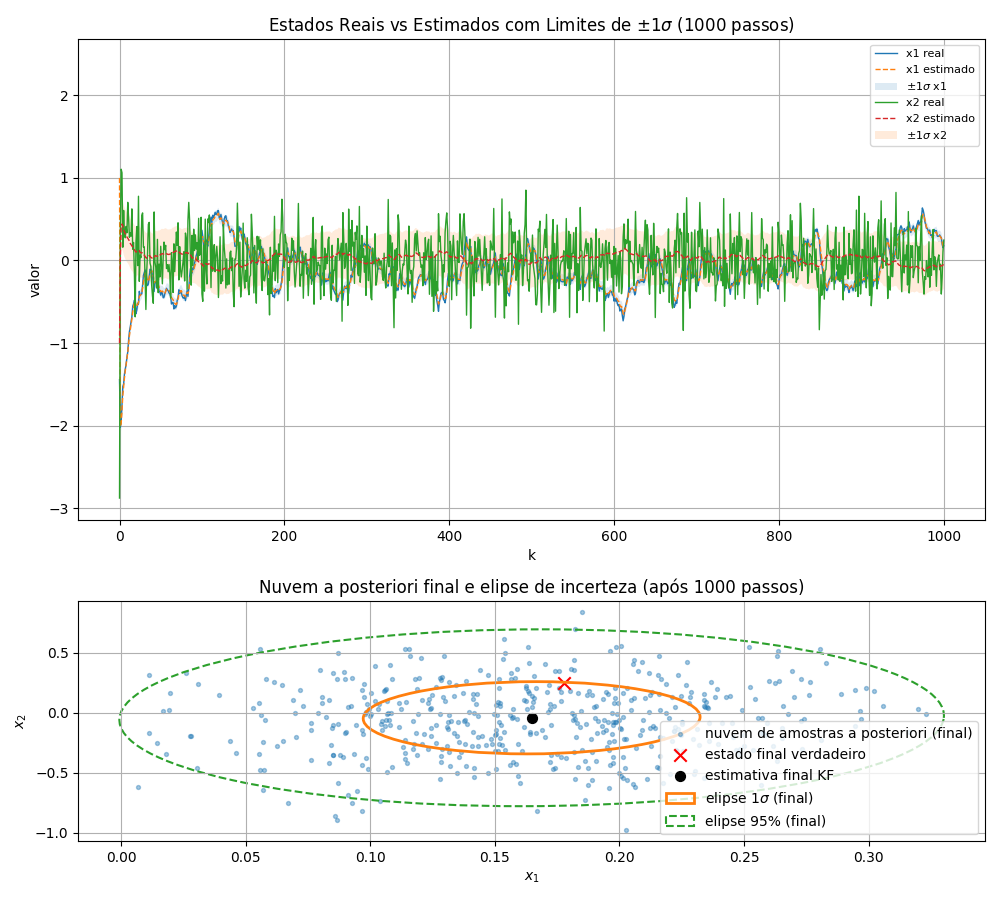
\includegraphics[width=\textwidth]{kf_resultados_1000_passos.png}
    \caption{Evolução do filtro de Kalman}
    \label{fig:kf_resultados_1000_passos}
\end{figure}

\section*{Questão 2}

\subsection*{a}

\ref{fig:chua_comparacao_vC1} mostra a comparação entre os dados coletados e a estimativa dos filtros EKF e UKF para a tensão $v_{C1}$.

\begin{figure}[H]
    \centering
    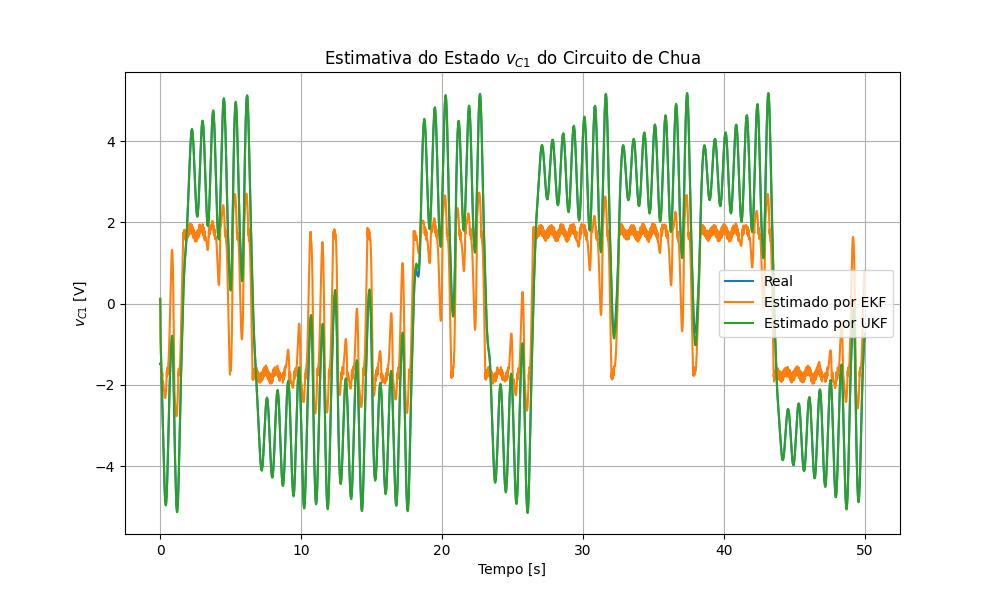
\includegraphics[width=\textwidth]{chua_comparacao_vC1.png}
    \caption{Comparação para $v_{C1}$}
    \label{fig:chua_comparacao_vC1}
\end{figure}

\subsection*{b}

\ref{fig:chua_comparacao_vC2_iL} mostra a comparação entre os dados coletados e a estimativa dos filtros EKF e UKF para a tensão $v_{C2}$ e corrente $i_{L}$.

\begin{figure}[H]
    \centering
    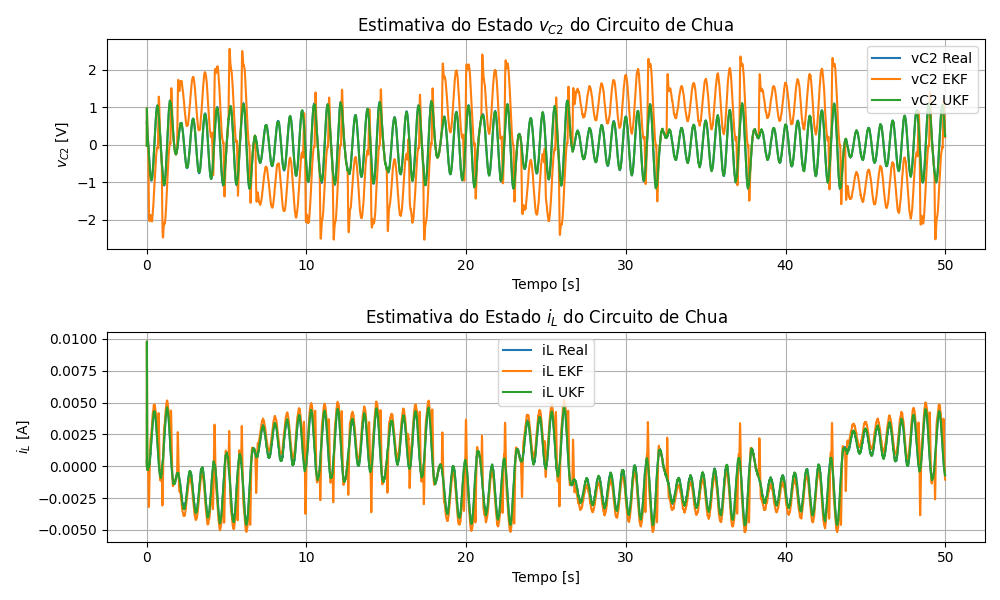
\includegraphics[width=\textwidth]{chua_comparacao_vC2_iL.png}
    \caption{Comparação para $v_{C2}$ e $i_{L}$}
    \label{fig:chua_comparacao_vC2_iL}
\end{figure}

\end{document}